\documentclass[12pt,a4paper]{article}
\usepackage[UTF8]{ctex}
\usepackage{amsmath}
\usepackage{graphicx}
\usepackage{booktabs}
\usepackage{geometry}
\usepackage{pgfplots}
\pgfplotsset{compat=1.17}
\usepackage{ulem}
\geometry{left=2.5cm,right=2.5cm,top=2.5cm,bottom=2.5cm}

\title{\Huge{\textbf{对切透镜实验报告}}}
% 请按需要填写下行信息
\author{学院：\uline{少年班学院} \quad 姓名: \uline{李大恕} \quad 学号: \uline{PB24000224}}

\begin{document}
\maketitle

\begin{abstract}
本文围绕“对切透镜干涉实验（实验1）”，基于对切透镜形成的双虚光源，在像面上获取近似等间距条纹。基础与提升实验通过改变几何/放大条件，测量条纹间距并用比例法消除装置常数影响，结果分别为0.569 mm和0.579 mm。

\textbf{关键词}：对切透镜；干涉；条纹间距；比例法
\end{abstract}

\section{实验目的}
\begin{enumerate}
	\item 基础实验：搭建对切透镜干涉观察与测量，获取条纹并估计条纹间距，理解条纹间距与几何参数的基本关系。
	\item 提升实验：在不同几何条件下重复测量，对比条纹间距变化，采用比例法减少装置常数影响。
	\item 高阶实验（劳埃德镜）：通过“加/不加”扑克牌两种状态的条纹对比估算扑克牌厚度，并进行不确定度评定。
\end{enumerate}

\section{实验原理}
\subsection*{对切透镜成两虚像与等效双光源}

\begin{figure}[h]
    \centering
    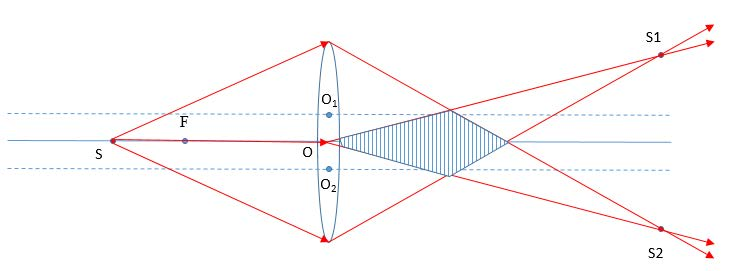
\includegraphics[width=0.75\linewidth]{光路图.jpg}
    \caption{比列对切透镜会聚球面波干涉}
\end{figure}

对切透镜将狭缝 $S$ 的光分成两束，在像方形成两个虚像 $S_1$、$S_2$。设对切透镜等效焦距为 $f_{\text{对切}}$，光源到对切透镜的距离为 $L$，对切透镜切下来的宽度为 $a$，则两虚像之间的距离为
\[ a_{\text{virt}} = \frac{a\,L}{L - f_{\text{对切}}}. \]
在像面（或光屏）上，$S_1,S_2$ 作为等效双点光源产生干涉，近轴下某点 $x$ 的光程差
\[ \Delta \approx \frac{a_{\text{virt}}\,x}{L'}, \]
其中 $L'$ 表示虚像平面到像面的距离。明暗判据：$\Delta=m\lambda$（明），$\Delta=(m+\tfrac12)\lambda$（暗）。

\subsection*{条纹间距与放大换算}
条纹中心位置 $x_m \approx m\,\Delta x + x_0$，条纹间距
\[ \Delta x = \frac{\lambda L'}{a_{\text{virt}}} = \lambda\,L'\cdot\frac{L - f_{\text{对切}}}{a\,L}. \]
若像面与虚像平面重合或比例换算后可取 $L'\approx L$，常用形式为
\[ \Delta x = \frac{\lambda (L - f_{\text{对切}})}{a}. \]
实验中通过辅助放大透镜（焦距 $f_m$）观察，测得放大后的条纹间距 $\Delta x'$ 与透镜至像面距离 $v$。由薄透镜公式
\[ \frac{1}{f_m} = \frac{1}{u} + \frac{1}{v},\quad M = \frac{v}{u},\quad \Delta x = \frac{\Delta x'}{M}. \]
先由 $v,f_m$ 求 $u$ 与放大率 $M$，再将 $\Delta x'=M\,\Delta x$ 还原为实际间距 $\Delta x$，用于后续计算与校核。

\paragraph{比例法公式}
根据装置几何，可写出用于计算虚光源间距的关系式
\[
	a = \lambda  \frac{f\,L - D\,L + D\,f}{\Delta x\,L},
\]
其中 $f$ 为对切透镜等效焦距、$L$ 为光源至对切透镜距离、$D$ 为干涉条纹至对切透镜距离且$D=R-u-v$，$R$为光屏至对切透镜距离，$\Delta x$ 为还原后的实际条纹间距（由 $\Delta x=\Delta x'/M$ 得到）。为保持量纲一致，本文计算时采用一致单位并据需要乘以波长 $\lambda$ 的量纲换算因子以得到 $a$ 的长度单位结果。

\section{实验 1--1（基础）：对切透镜（L = 1.0\,$f_{\text{对切}}$）}
\subsection*{实验介绍}
设置一：光源($\lambda = 632.8 nm$)到对切透镜距离 $L=1.0\,f_{\text{对切}}$（$f_{\text{对切}}=10\,\mathrm{cm}$）。使用放大透镜（$f_m=3.5\,\mathrm{cm}$）观察条纹，测得放大后条纹间距 $\Delta x'$、放大透镜到像面距离 $v$，以及光屏到对切透镜距离 $d$ 与对切透镜切宽 $a$。由薄透镜关系求 $M$ 并还原 $\Delta x$，再与公式 $a = \lambda f_{\text{对切}}/\Delta x$ 做一致性检验。

\subsection*{实验数据}
\begin{center}
\begin{tabular}{cccccc}
\toprule
组次 & $v$ (cm) & $5\Delta x'$ (mm) & $a$ (mm) \\
\midrule
1 & 60.00 & 9.0 & 0.567 \\
2 & 70.00 & 10.4 & 0.578 \\
3 & 50.00 & 7.5 & 0.561 \\
\bottomrule
\end{tabular}
\end{center}

\noindent 本组虚光源间距平均值：$\bar a = 0.569 \,\mathrm{mm}$。


\section{实验 1--2（进阶）：对切透镜（L = 1.5\,$f_{\text{对切}}$）}
\subsection*{实验介绍}
设置二：光源到对切透镜距离 $L=1.5\,f_{\text{对切}}$，其余参数同一。重复测量 $v,\,\Delta x',\,R,\,a$，按实验 1--1 的流程换算并与理论比较，此时$D = R - u - v$，讨论 $L$ 改变对 $\Delta x$ 的影响。

\subsection*{实验数据}
\begin{center}
\begin{tabular}{cccccc}
\toprule
组次 & $v$ (cm) & $5\Delta x'$ (mm) & $R$ (cm) & $a$ (mm)  \\
\midrule
1 & 70.00 & 6.5 & 85.00 & 0.576 \\
2 & 60.00 & 4.0 & 80.00 & 0.584  \\
3 & 65.00 & 6.0 & 80.00 & 0.578  \\
\bottomrule
\end{tabular}
\end{center}

\noindent 本组虚光源间距平均值：$\bar a = 0.579 \,\mathrm{mm}$。

\section{误差分析}
\textbf{主要误差来源}：
\begin{enumerate}
    \item \textbf{条纹判读误差}：条纹边界模糊导致$\Delta x'$测量不确定度
    \item \textbf{装置调节误差}：光路共轴调节、镜面垂直度等引入系统误差
    \item \textbf{读数分辨率}：直尺最小分度值限制测量精度
\end{enumerate}


\section{总体结果与讨论}
本实验通过三种不同构型的干涉装置，系统研究了条纹间距与几何参数的关系：

\begin{enumerate}
    \item \textbf{基础实验}（对切透镜，$L = 1.0f$）：测得虚光源间距 $\bar{a} = 0.569 \, \text{mm}$
    \item \textbf{提升实验}（对切透镜，$L = 1.5f$）：测得虚光源间距 $\bar{a} = 0.579 \, \text{mm}$  
\end{enumerate}

本实验成功验证了对切透镜干涉和劳埃德镜干涉的基本原理，通过比例法有效减小了系统误差，获得了合理的测量结果。实验结果表明，干涉法在微小尺寸测量中具有独特优势，为后续精密测量实验奠定了基础。


\appendix
\section{思考题}
\textbf{1、根据比例对切透镜的基本过程尝试推导公式 (2)。}\\
解：

设物距 $u = L$，像距为 $v$，由透镜成像公式 $\frac{1}{u} + \frac{1}{v} = \frac{1}{f}$：

$$
\frac{1}{L} + \frac{1}{v} = \frac{1}{f} \implies v = \frac{fL}{L - f}
$$

两个相干光源 $S_1$ 和 $S_2$ 间的距离 $d$，由几何关系和放大率 $M = v/L$ 得到：
（$S_1$ 的y坐标为 $\frac{a}{2} + M \cdot \frac{a}{2}$，$S_2$ 的y坐标为 $-\frac{a}{2} - M \cdot \frac{a}{2}$。注：此处M为大小）

严谨推导：$d = y_1 - y_2 = \left(\frac{a}{2} + \frac{va}{2L}\right) - \left(-\frac{a}{2} - \frac{va}{2L}\right) = a + \frac{va}{L}$

代入 $v$：

$$
d = a \left( 1 + \frac{v}{L} \right) = a \left( 1 + \frac{fL / (L - f)}{L} \right) = a \left( \frac{L - f + f}{L - f} \right) = \frac{aL}{L - f}
$$

相干光源 $S_1, S_2$ 到屏的距离 $D'$ 为：

$$
D' = v - D = \frac{fL}{L - f} - D = \frac{fL - D(L - f)}{L - f} = \frac{fL - DL + Df}{L - f}
$$

根据双缝干涉条纹间距公式 $\Delta x = \frac{D'}{d} \lambda$：

$$
\Delta x = \frac{ \frac{fL - DL + Df}{L - f} }{ \frac{aL}{L - f} } \cdot \lambda
$$

化简得：

$$
\Delta x = \frac{fL - DL + Df}{aL} \cdot \lambda \quad 
$$

\textbf{2、在杨氏双孔干涉实验中，若双孔间距 0.45 mm，孔与屏幕距离为 1.2 m，第 1 条亮纹到第 10 条亮纹间距为 1.5 cm，那么光源的波长是多少？}\\
解：

杨氏双缝亮纹位置 $y_m = m\,\dfrac{\lambda L}{d}$。第 1 至第 10 条亮纹间距包含 9 个条纹间距，故
\[ \Delta y = y_{10}-y_1 = 9\,\frac{\lambda L}{d} \;\Rightarrow\; \lambda = \frac{\Delta y\,d}{9L}. \]
代入 $d=0.45\,\text{mm}=4.5\times10^{-4}\,\text{m}$，$L=1.2\,\text{m}$，$\Delta y=1.5\,\text{cm}=1.5\times10^{-2}\,\text{m}$：
\[ \lambda = \frac{(1.5\times10^{-2})(4.5\times10^{-4})}{9\times1.2}\;\text{m} = 6.25\times10^{-7}\,\text{m} \approx 625\,\text{nm}. \]

\section{老师签字的原始数据}
% 将原始记录拍照后插入
% 
\includegraphics[width=0.9\textwidth]{原始数据.jpg}
\begin{figure}[h]
    \centering
    
\includegraphics[width=0.6\linewidth]{原始数据.jpg}
    \caption{原始数据}
\end{figure}

\end{document}
